% $Id: template.tex 11 2007-04-03 22:25:53Z jpeltier $

\documentclass{vgtc}                          % final (conference style)
%\documentclass[review]{vgtc}                 % review
%\documentclass[widereview]{vgtc}             % wide-spaced review
%\documentclass[preprint]{vgtc}               % preprint
%\documentclass[electronic]{vgtc}             % electronic version

%% Uncomment one of the lines above depending on where your paper is
%% in the conference process. ``review'' and ``widereview'' are for review
%% submission, ``preprint'' is for pre-publication, and the final version
%% doesn't use a specific qualifier. Further, ``electronic'' includes
%% hyperreferences for more convenient online viewing.

%% Please use one of the ``review'' options in combination with the
%% assigned online id (see below) ONLY if your paper uses a double blind
%% review process. Some conferences, like IEEE Vis and InfoVis, have NOT
%% in the past.

%% Figures should be in CMYK or Grey scale format, otherwise, colour 
%% shifting may occur during the printing process.

%% These few lines make a distinction between latex and pdflatex calls and they
%% bring in essential packages for graphics and font handling.
%% Note that due to the \DeclareGraphicsExtensions{} call it is no longer necessary
%% to provide the the path and extension of a graphics file:
%% \includegraphics{diamondrule} is completely sufficient.
%%
\ifpdf%                                % if we use pdflatex
  \pdfoutput=1\relax                   % create PDFs from pdfLaTeX
  \pdfcompresslevel=9                  % PDF Compression
  \pdfoptionpdfminorversion=7          % create PDF 1.7
  \ExecuteOptions{pdftex}
  \usepackage{graphicx}                % allow us to embed graphics files
  \DeclareGraphicsExtensions{.pdf,.png,.jpg,.jpeg} % for pdflatex we expect .pdf, .png, or .jpg files
\else%                                 % else we use pure latex
  \ExecuteOptions{dvips}
  \usepackage{graphicx}                % allow us to embed graphics files
  \DeclareGraphicsExtensions{.eps}     % for pure latex we expect eps files
\fi%

%% it is recomended to use ``\autoref{sec:bla}'' instead of ``Fig.~\ref{sec:bla}''
\graphicspath{{figures/}{pictures/}{images/}{./}} % where to search for the images
\usepackage{float}
\usepackage{microtype}                 % use micro-typography (slightly more compact, better to read)
\PassOptionsToPackage{warn}{textcomp}  % to address font issues with \textrightarrow
\usepackage{textcomp}                  % use better special symbols
\usepackage{mathptmx}                  % use matching math font
\usepackage{times}                     % we use Times as the main font
\renewcommand*\ttdefault{txtt}         % a nicer typewriter font
\usepackage{cite}                      % needed to automatically sort the references
\usepackage{tabu}                      % only used for the table example
\usepackage{booktabs}                  % only used for the table example
%% We encourage the use of mathptmx for consistent usage of times font
%% throughout the proceedings. However, if you encounter conflicts
%% with other math-related packages, you may want to disable it.


%% If you are submitting a paper to a conference for review with a double
%% blind reviewing process, please replace the value ``0'' below with your
%% OnlineID. Otherwise, you may safely leave it at ``0''.
\onlineid{0}

%% declare the category of your paper, only shown in review mode
\vgtccategory{Research}

%% allow for this line if you want the electronic option to work properly
\vgtcinsertpkg

%% In preprint mode you may define your own headline.
%\preprinttext{To appear in an IEEE VGTC sponsored conference.}

%% Paper title.

\title{Interfacing with Leap Motion Controller to Virtually Create Digital Music}

%% This is how authors are specified in the conference style

%% Author and Affiliation (single author).
%%\author{Roy G. Biv\thanks{e-mail: roy.g.biv@aol.com}}
%%\affiliation{\scriptsize Allied Widgets Research}

%% Author and Affiliation (multiple authors with single affiliations).
%%\author{Roy G. Biv\thanks{e-mail: roy.g.biv@aol.com} %
%%\and Ed Grimley\thanks{e-mail:ed.grimley@aol.com} %
%%\and Martha Stewart\thanks{e-mail:martha.stewart@marthastewart.com}}
%%\affiliation{\scriptsize Martha Stewart Enterprises \\ Microsoft Research}

%% Author and Affiliation (multiple authors with single affiliations).
\author{DeAnn M. Jones\thanks{e-mail:djone010@colostate.edu}\\ %
     \parbox{1.4in}{\scriptsize \centering Computer Science Department \\ Colorado State University}}

%% A teaser figure can be included as follows, but is not recommended since
%% the space is now taken up by a full width abstract.
%\teaser{
%  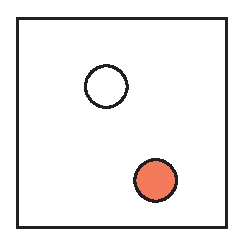
\includegraphics[width=1.5in]{sample.eps}
%  \caption{Lookit! Lookit!}
%}

%% Abstract section.
\abstract{
Since the 1950s, artists and composers have been experimenting with computing technology as a medium to create digital art and music. In recent years, technological advances in motion detection sensor hardware and software have reached new heights allowing for immersive interaction with virtual environments. This research paper will discuss the use of Ultraleap, Inc.’s hand tracking technology known as, Leap Motion controller, in order to give users an alternative and technologically innovative platform to create music. This paper covers previous research regarding digital music and virtual instruments, describes the development of a prototype virtual guitar, includes a project research experiment, and also discusses future feature enhancements and functional improvements of the Leap Motion Guitar prototype.
} % end of abstract

%% ACM Computing Classification System (CCS). 
%% See <http://www.acm.org/class/1998/> for details.
%% The ``\CCScat'' command takes four arguments.

\CCScatlist{ 
  Leap Motion, Unity game engine, music and musical theory education, virtual guitar.
}

%% Copyright space is enabled by default as required by guidelines.
%% It is disabled by the 'review' option or via the following command:
% \nocopyrightspace

%%%%%%%%%%%%%%%%%%%%%%%%%%%%%%%%%%%%%%%%%%%%%%%%%%%%%%%%%%%%%%%%
%%%%%%%%%%%%%%%%%%%%%% START OF THE PAPER %%%%%%%%%%%%%%%%%%%%%%
%%%%%%%%%%%%%%%%%%%%%%%%%%%%%%%%%%%%%%%%%%%%%%%%%%%%%%%%%%%%%%%%%

\begin{document}

%% The ``\maketitle'' command must be the first command after the
%% ``\begin{document}'' command. It prepares and prints the title block.

%% the only exception to this rule is the \firstsection command
\firstsection{Introduction}

\maketitle

%% \section{Introduction} %for journal use above \firstsection{..} instead
With the invention of the digital transistor and integrated circuits in the 20th century, traditional musical instruments evolved into novel, unprecedented formats capable of creating iconic sounds such as, the digital synthesizer and the electronic guitar. Also in the late 20th century, there was much growth in the study of human motion in biometrics. This type of study included the work of Dr. Tom Calvert, a leading technology professor in the study of computer science and kinesiology at that time. Dr Calvert created what was known as, potentiometers, which were computer sensors capable of tracking flexes and extensions of the human knee \cite{Calvert:1982:AKS}. 

Soon after this, the Massachusetts Institute of Technology developed an optical motion capture system that rendered an actor’s movements in two dimensions \cite{Maxwell:1984:GM}. In recent years, motion detection hardware sensors and software have become widely used in a large range of industries, especially the computer gaming industry, where such devices are used to interact with objects within virtual environments.

\begin{figure}[h]
\centering
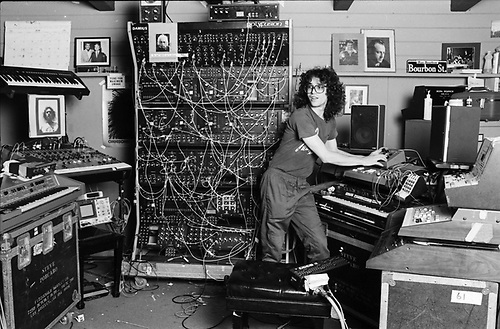
\includegraphics[width=5cm]{pictures/Steve_Porcaro.jpg}
\centering
\caption{1982 photo of digital synthesizer instrumentalist Steve Porcaro from the popular rock band Toto performing the hit song Africa in his home studio. The image was found in the public domain}
\end{figure}

This project builds upon multiple decades of this previous work and primarily focuses on the development of a virtual guitar system. The Leap Motion Guitar prototype uses the Unity game engine in order to provide interactive visual feedback. The Leap Motion Guitar prototype also utilizes an optical hand tracking hardware sensor called, Ultraleap Leap Motion controller, as a means of acquiring hand motion input. 

To create music, a musician just holds their hands above the Leap Motion controller (the independent variable), which is placed directly in front of the computer keyboard. Their hand movements (the dependent variable) are visually reflected on the computer screen, where they can provide chord numbers on the fingers of one hand, while strumming the virtual guitar with their other hand. This type of research has a wide variety of practical uses such as, in the education of music and music theory. This type of research may possibly, one day, replace the need for physical musical instruments with these new virtual forms.

\begin{figure}[h]
\centering
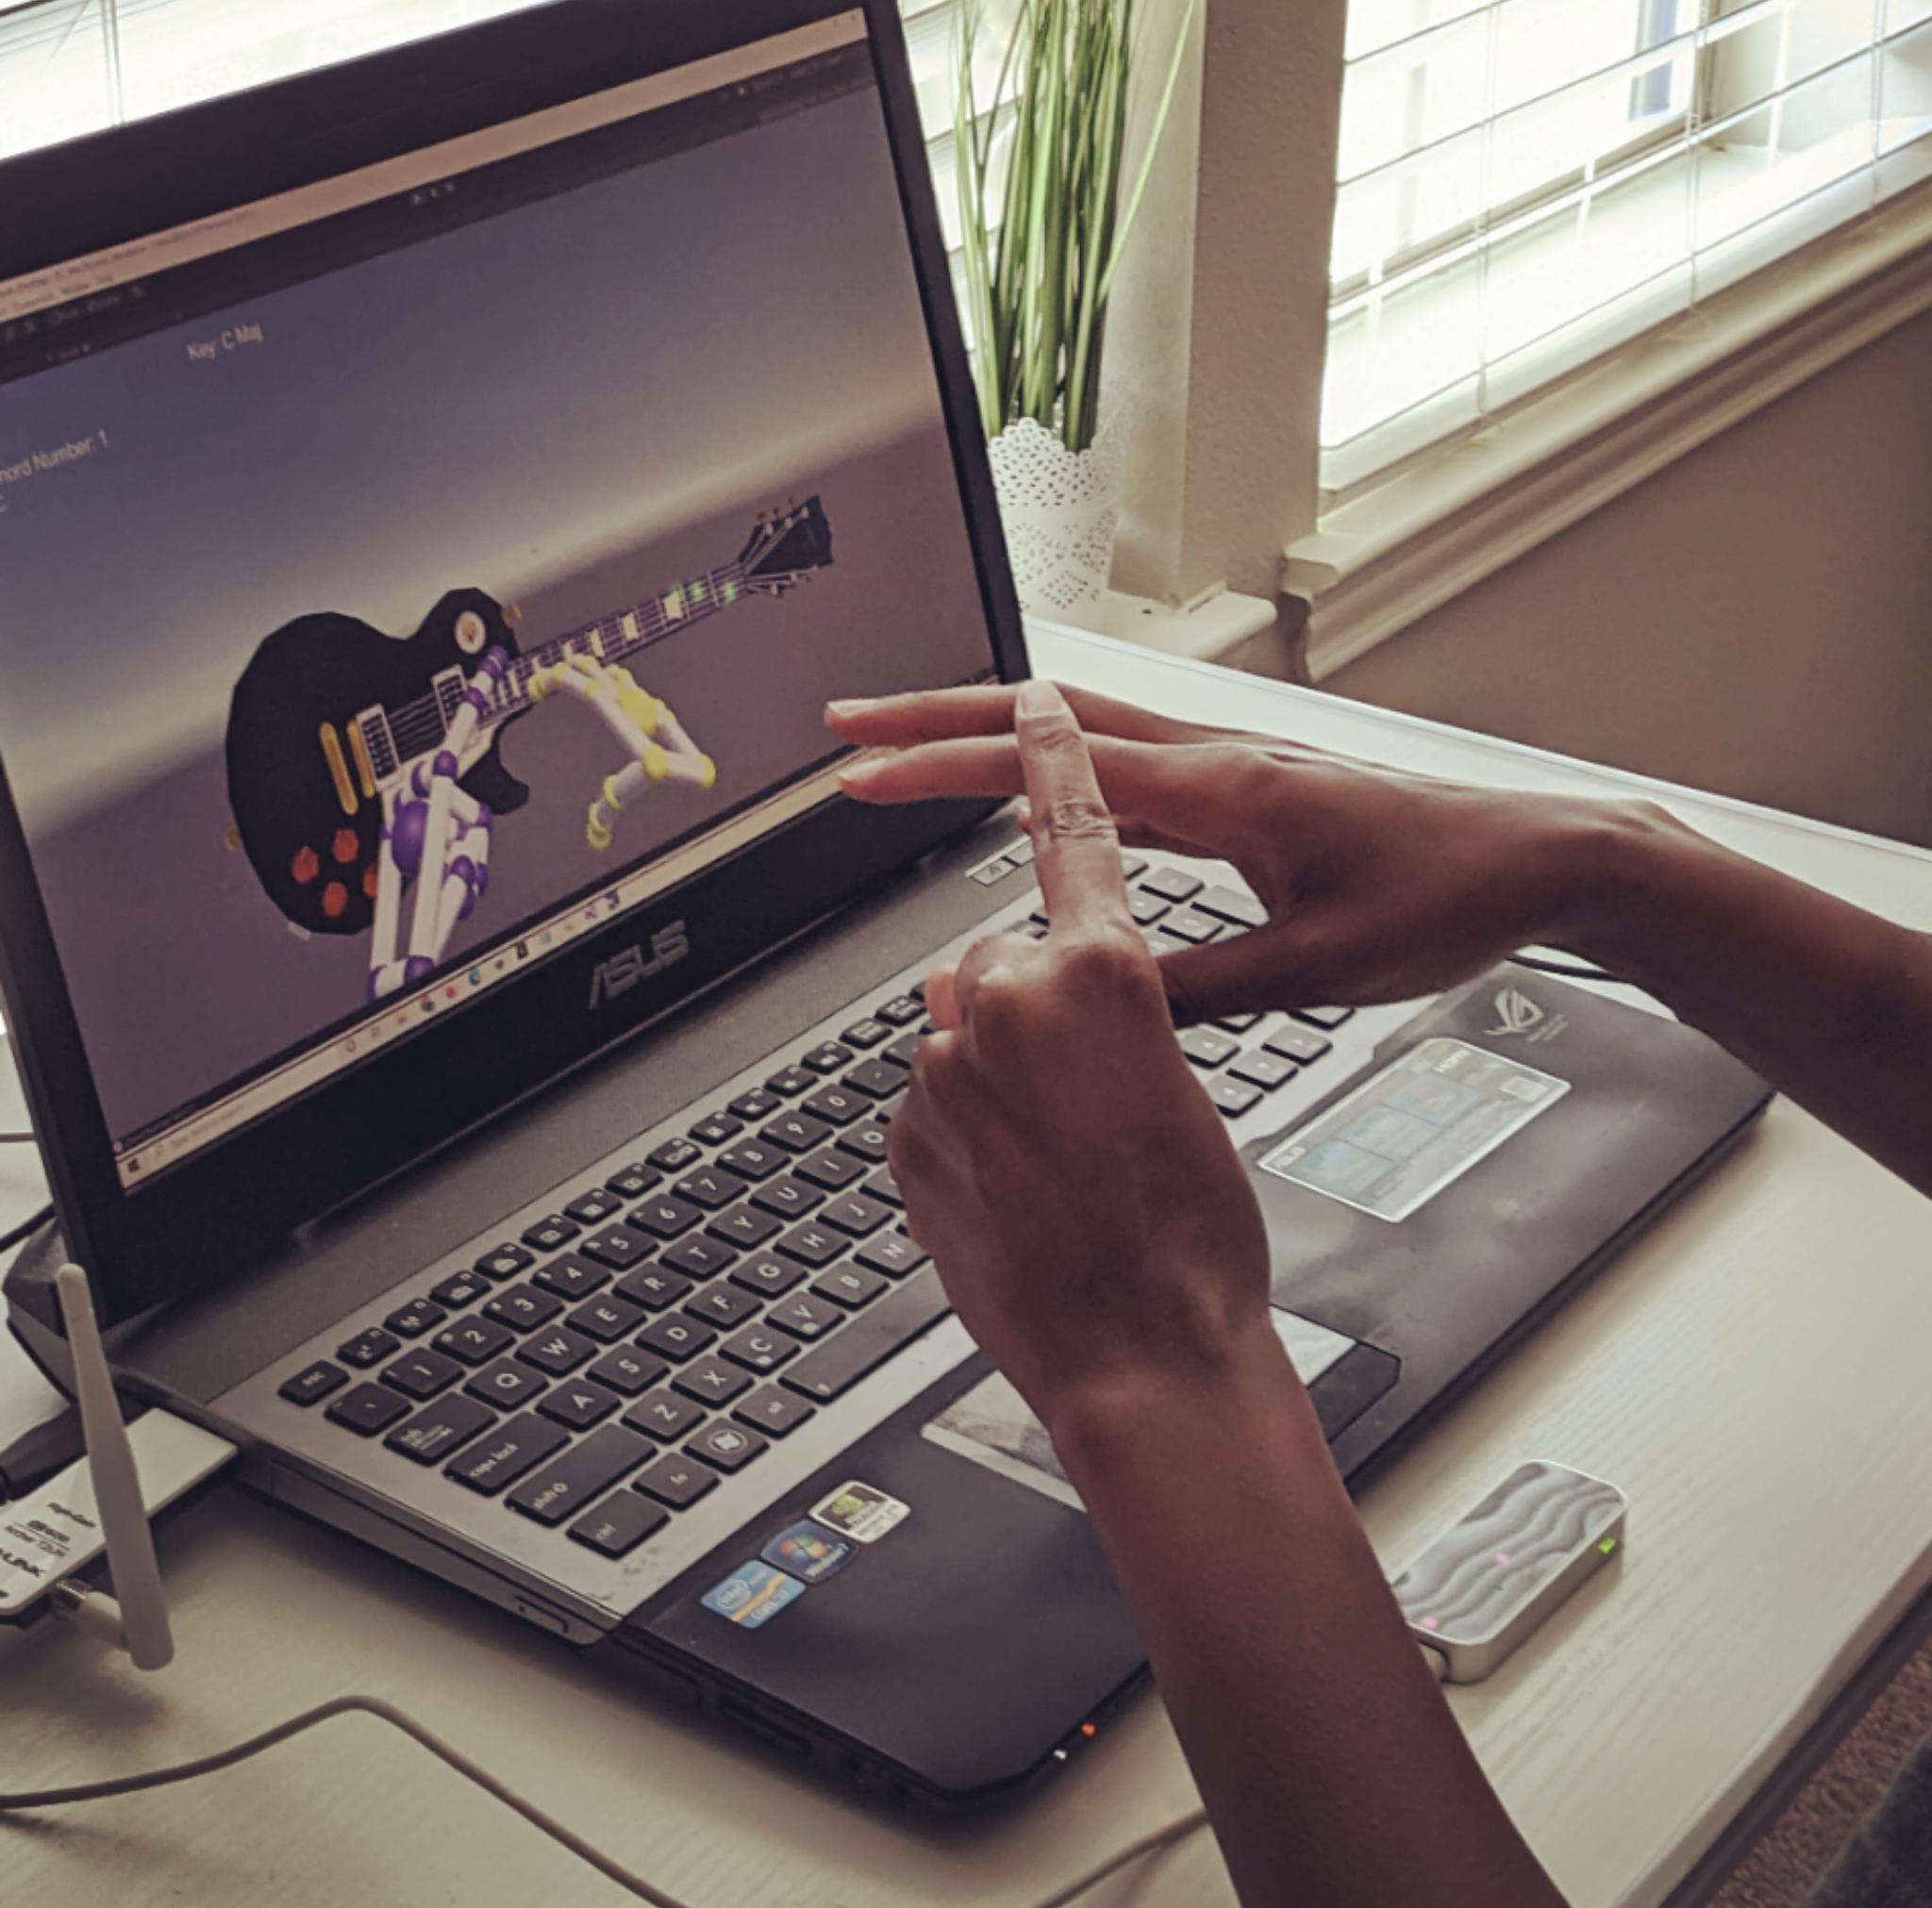
\includegraphics[height=4cm]{pictures/Leap_Motion_Guitar_Jones.png}
\centering
\caption{ Jones demonstrates using the Ultraleap Leap
Motion controller to interact with the virtual guitar in Unity}
\end{figure}

There is also a high motivation for this type of research: the ability to fill the need for those who enjoy making music but are economically or physically unable. Statistical evidence has correlations between the positive influence music has on cognitive skills and IQ. Unfortunately, many individuals worldwide live in poverty and cannot afford instruments or associated training; thus, they cannot reap the benefit of learning basic music theory. Along with addressing accessibility needs, this research could potentially address the needs of those with physical impairments concerning creating music. For some, hauling or handling musical equipment can be strenuous or completely unachievable due to a physical impairment. For these marginalized individuals, this research hopes to offer alternative avenues for making music.

\section{Related Work}

Various limitations of creating traditional music have led artists and composers to explore the digital generation of music through computer and MIDI technology. This is primarily because traditional musical instruments are limited to a small variety of timbres, a low range of tones and pitches, as well as only supporting a small amount of performance forms such as, hitting, strumming, pulling, and blowing air into physical objects. Applying computer music production models removes these limitations, but also allows composers to more efficiently create the scoring, orchestration, and performance of their work. The use of computer technology improves the performer's comprehension and understanding of the composer's work and vastly saves on human, material, and financial costs and resources burdened by traditional music creation \cite{Liang:2021:RAD}.

In the last two decades, traditional means of human machine interface, through computer mouse and keyboard, have evolved into touch-less interface technologies. In the early 2000s, wearable glove-like devices were developed using various hardware sensors that were attached to the hands and fingers.  These devices were capable of detecting various degrees of flexing and bending of five fingers as well as detecting hand orientation \cite{Chong:2018:ASL, Kevin:2004:TMI}. Due to the low data resolution and lack of precision of these sensor-based devices, researchers began to experiment with utilizing machine learning and neural network training technology in order to provide low latency and high accuracy hand gesture recognition \cite{Nguyen:2013:SHG}. Building on this research into machine learning hand gesture recognition, many successful commercial products have become available such as, the Microsoft Kinect, Sony PlayStation Eye, Ultraleap Leap Motion controller and the more recent Oculus Quest VR headset. These hardware devices are capable of capturing and translating real-time video frames of hand motions and convert them into three dimensional computer models \cite{Rautaray:2012:VBH, Chen:2020:GCM}.

\begin{figure}[h]
\centering
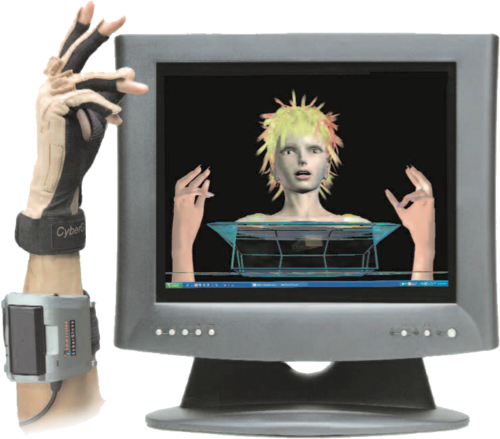
\includegraphics[width=4cm]{pictures/cyber-glove-2.png}
\centering
\caption{The Cyberglove-II was an early sensor-based approach at hand gesture recognition. Image available at http://www.cyberglovesystems.com/cyberglove-ii}
\end{figure}

Now that real-time gesture recognition was possible, modern computer vision interface devices were positioned to have a large impact on the creation of digital music. Using these low cost and portable devices capable of both visualization and gesture recognition, researchers began to develop virtual reality musical instruments. One such device developed in 2015 was known as Wedge, which combined the Oculus Rift headset with a Leap Motion controller. Wedge provided a musical interface where a musician would compose virtual music via arranging virtual rectangle blocks assigned with pitches and MIDI note numbers. Once the "build" session was complete, the performer could then "play" the arranged music. Another device known as ChromaChord was also developed in this same year with the same technologies. In this type of immersive 3-D environment, musicians were able to create live music by making grab-and-point gestures in order to synthesize melodic sequences of sounds \cite{Serafin:2016:VRM}. Recently, an application known as, Experience Ochestra and created for the Oculus Quest 2, allows a musician the ability to virtually play sixteen musical instruments, including the violin and french horn, without requiring the knowledge to physically play these instruments \cite{Choi:2022:EOM}.
\begin{figure}[H]
\centering
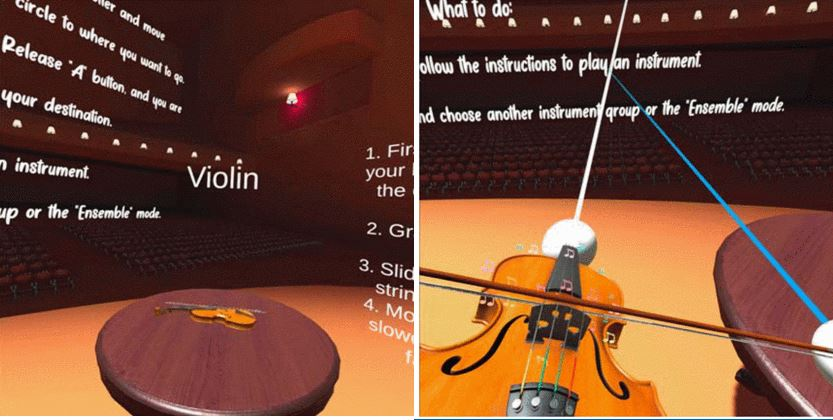
\includegraphics[height=4cm]{pictures/experience-orchestra-violin.JPG}
\centering
\caption{Screenshot of a user playing the Experience Orchestra violin for Oculus Quest \cite{Choi:2022:EOM}}
\end{figure}
\section{Methodology}

This Leap Motion Guitar prototype project demonstrates and explores gesture and motion-based digital music applications and their potential capabilities. The prototype also suggests a possible user interface design to create guitar music through hand motions and gestures. Because the controller is capable of sensing hand and finger motions as input analogous to a mouse, it requires no physical contact or touching. In addition to the Unity Game Engine itself, the only other software that was required was the Leap Motion Unity Plugin. The initial functionality of the prototype involves using basic finger gestures representing chord progression numbers on one hand while making strumming gestures on the other.  

To achieve this, the guitar model is capable of detecting strumming patterns when the Leap Motion hand models intersect a three dimensional capsule collider located on the model itself, where the virtual strings are located. This trigger then initiates specific guitar chord audio, which is determined by the chord number gestured by the left hand. The Leap Motion controller API provides C Sharp scripts capable of providing the left hand motion states of which fingers are extended and which are not extended.

\begin{figure}[h]
\centering
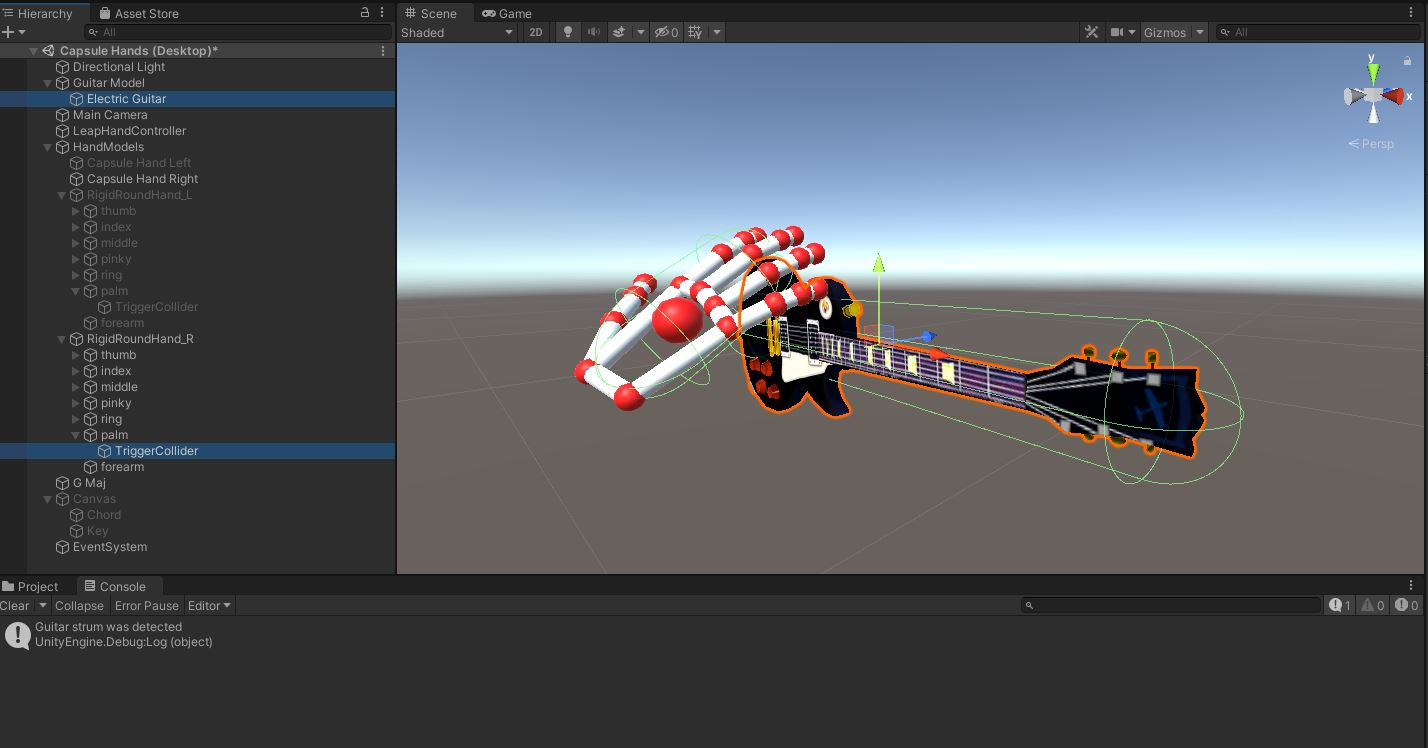
\includegraphics[width=7cm, height=4cm]{pictures/Capsule_Collider.JPG}
\centering
\caption{A three dimensional model of a guitar displaying collision detection capsules added in Unity in order to aid in the detection of strumming motion on the virtual guitar model. Image taken by Jones.}
\end{figure}

The Leap Motion Guitar prototype focuses on the musical key of C major. Because the majority of popular songs only utilize the first five chords in a key, this project only focuses on producing specific guitar chord audio from the subset of C major which are as follows:

\begin{enumerate}
  \item C major(C)
  \item D minor(Dm)
  \item E minor(Em)
  \item F major(F)
  \item G major(G)
\end{enumerate}

As the musician's left hand presents chord number gestures, the user interface (UI) displays the chord number as well as the chord name as text on the screen. In addition to this visual feedback, which lets the musician know the correct chord will sound as intended, the fret board on the virtual guitar neck contains colored LED lights for learning purposes. This conveys the actual finger placements needed to create the chord if the user were to play a standard tuned actual guitar.

\begin{figure}[H]
\centering
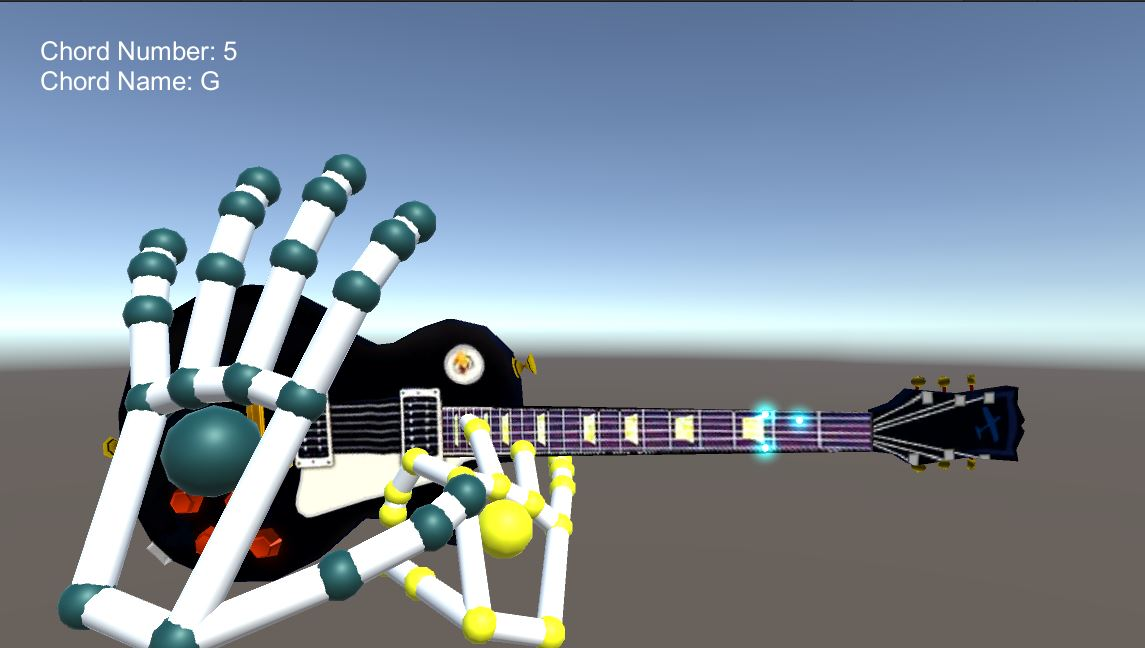
\includegraphics[height=4cm]{pictures/Strumming_with_chord_number.JPG}
\centering
\caption{This figure shows left hand chord five detected as G Major with blue LED indicators on the guitar neck representing which strings and frets one would push down on an actual guitar. Image taken by Jones.}
\end{figure}

\section{Experiment Design}

During the experiment, usability and functionality of the prototype was measured. To measure these criteria, the participants chosen varied in age, gender, and musical experience. Each of the 10 participants were instructed, one by one, to first strum the C major chord using the Leap Motion virtual guitar prototype. Then, the participant was asked to strum the D minor, E minor, F major, and G major chords, one after the other using the left hand chord number gestures. After this, the participant was instructed to play the children's song, "Twinkle, Twinkle, Little Star" which was provided on the corresponding sheet music in Figure 7. 

\begin{figure}[H]
\centering
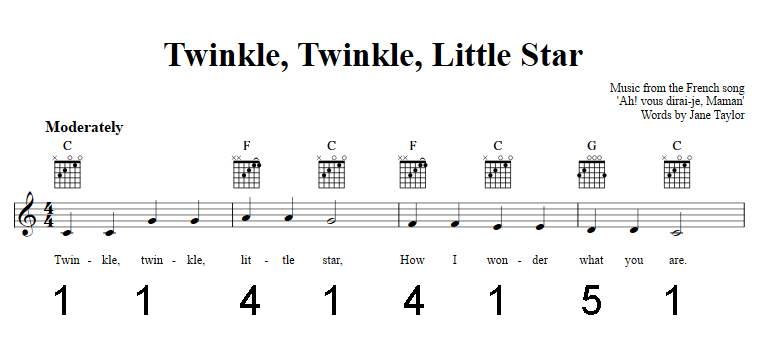
\includegraphics[height=4cm]{pictures/ttlstar-sheet-music.png}
\centering
\caption{Sheet music for Twinkle Twinkle Little Star provided to experiment participants.  Sheet music found in public domain and modified by Jones to include chord progression numbers.}
\end{figure}

An unlimited amount of time was allowed to complete one attempt of the exercise. After the attempt was completed, the participant was asked to complete an 8-question survey regarding their prior musical experience, age, gender, and their ability to play the piece. The survey additionally gathered their opinions on the future of virtual reality musical instruments, and also gathered valuable opinions on possible future enhancements to the prototype.

For this experiment, my hypotheses are as follows:
\begin{itemize}
    \item Of the 10 randomly selected participants, 90\% of them will have at least moderate musical knowledge (a 3 or higher on the "musical skill level" scale of 1-10).   
    \item Over 80\% of the participant pool will be able to play all five chords offered on the virtual guitar prototype with no difficulty.
    \item Over 70\% of the participant pool will be able to play the children's song provided with no difficulty.
\end{itemize}

\section{Results}
Within the sample of 10 participants, 40\% were female, 30\% were male, 10\% were non-binary, and the remaining 10\% chose not to state their gender. The dominating age of the group was between 36 and 45 years of age and comprised 30\% of the participant sample. 20\% of the participants were between 18 and 25 years of age; 20\% were between the ages of 26 and 35; 20\% were under the age of 18; 10\% were 45 or older. 20\% of the participants had no musical experience, 30\% had some to moderate experience, while 40\% were very musically inclined. Only 10\% of the participants were professional musicians. Based on these percentages, the average skill level amongst the participant pool was 4.8. This means that the overall skill level was slightly less than moderate, with a standard deviation 3.341.

\begin{figure}[h]
\centering
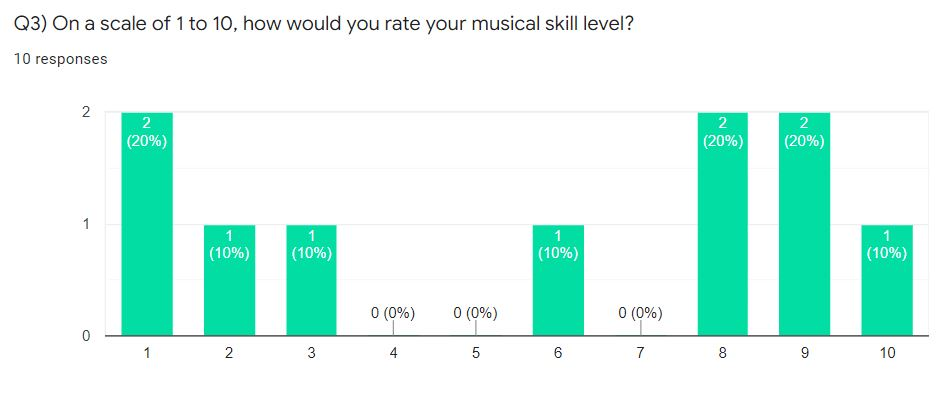
\includegraphics[width=8cm]{pictures/Survey_Skill_Level_Q3.JPG}
\centering
\caption{Survey results graph displaying participants' self-reported musical skill level.}
\end{figure}

When asked to play five chords offered on the virtual guitar prototype, 70\% of the participants had no difficulty at all. 20\% could still complete this task, but with some difficulty; 10\% could not complete the task at all. When asked to play the sheet music of the children's song, "Twinkle, Twinkle, Little Star," 40\% were able to play it without difficulty, while another 40\% played the song with some difficulty. 20\% could not play the song at all. After the task portion of the experiment, participants were asked the likelihood of this type of technology being prevalent in the future. 30\% believed that this technology's prevalence would not be very likely. Another 30\% of the participants moderately believed that this technology would be prevalent. 40\% believed technology like the Leap Motion Guitar prototype would be extremely likely to be prevalent. 

With this, the average was a 7 on the scale of prevalence, meaning that participants were generally confident that this type of technology will be prevalent in the future (Standard deviation of 2.996). Participants were then asked if they would like to see this type of technology in the future. 70\% said that they would like to see this type of technology in the future, while the remaining 30\% would not.

In the last question, participants were asked involved general feedback surrounding potential improvements that could be added to the Leap Motion Guitar prototype. Some of the participants wanted to be able to play the virtual guitar in VR, to provide a more realistic experience. Many of the participants enjoyed the prototype and wanted to see more options of keys available and various types of virtual instruments. 

\section{Limitations}
Some limitations were observed as participants carried out the experiment. One of the limitations included the way in which the strumming of the virtual guitar appeared on screen to the participant. The prototype requires users to strum the virtual guitar using a downward open-handed motion, while their hands hovered over the Leap Motion Controller.  Because the prototype only has a fixed camera in front of the guitar, the strumming motion reflected on the screen shows the virtual hands in front of the virtual guitar, instead of the true perspective of the user being behind the guitar.  Strumming in a more natural motion like one would have if they had a physical guitar could be acquired using an actual virtual reality headset.

Another limitation observed was the reactionary movement of the virtual hands to that of the participant's. Many of the participants had to adjust to the way in which the Leap Motion Controller picked up the motions of their hands. For example, when a participant attempted to make gestures indicating a desired number and corresponding chord, the virtual hands would contort and glitch until the participant patiently adjusted their fingers in a manner appropriate for the Leap Motion Controller to decipher the number.

\begin{figure}[h]
\centering
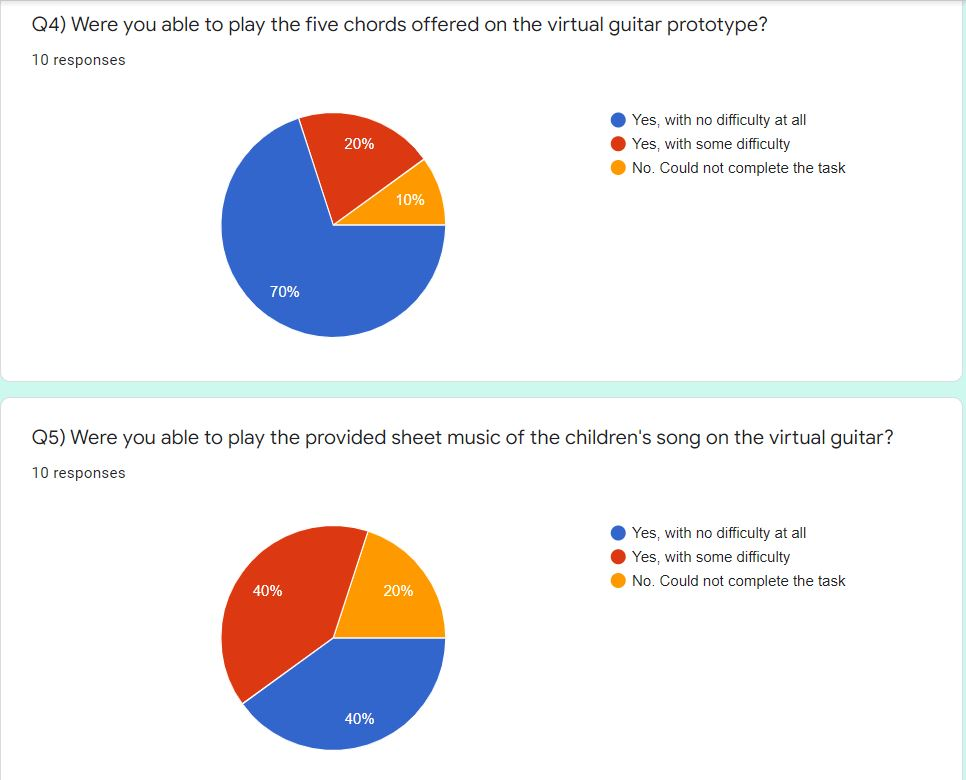
\includegraphics[height=7cm]{pictures/Survey_Difficulty.JPG}
\centering
\caption{Survey results displaying participants' difficulty completing tasks.}
\end{figure}

A follow-on prototype may help the user further if it were capable of displaying the virtual guitar in a perspective where the user's natural strumming view and motion could be perceived via a virtual reality headset.  This may assist the user in proper hand placement and positioning when teaching how to play songs on a virtual guitar.

\section{Conclusion}
My hypothesis, of at least 90\% of the participants having moderate musical knowledge, proved to be incorrect, as only 70\% had moderate musical knowledge. Furthermore, my hypothesis of the 80\% of participants being able to play the five chords without difficulty proved to be incorrect, while only 70\% were able to complete the task without difficulty. Even less were able to play the children's song without difficulty (40\%), proving my third hypothesis to also be incorrect. 

The gender and age had no effect on the participant's musical aptitude or ease of playing the musical pieces they were tasked with. A vast amount of the participants could play the five chords created for this experiment; however, playing a song proved to be slightly more difficult. Some could see this type of technology being prevalent in the future, and a vast majority would enjoy seeing things like the Leap Motion Guitar prototype in the future.  

The Leap Motion Guitar prototype allows musicians visual exposure and ability to interact with a virtual guitar. The user is able to produce music without requiring the knowledge of how to truly play the instrument and in doing so, learns actual musical theory involving chord progression numbers. The user is also able to learn chord finger positions on a standard guitar tuning. Future additions to the prototype could include more advanced hand gestures more closely related to playing traditional guitar chords as well as possible gestures for advanced chords. 

Since the experiment participants expressed difficulty with simple hand gestures, these features may be beyond the capabilities and data resolution output of the Leap Motion Controller device. I hope that the findings of this experiment will further other works that help those with disabilities or low socioeconomic status benefit from what music has to offer. Furthermore, I hope that the limitations  of this experiment will influence more advocacy for this type of technology.

%% if specified like this the section will be committed in review mode
\acknowledgments{
Thank you to the Unity Game Engine development team as well as the developers at Ultraleap for producing low cost, quality products so that students like myself can quickly learn to develop and produce modern software applications.

Thank you to the 10 participants that voluntarily demoed the Leap Motion Guitar prototype.

I also would like to thank my husband Jonah for providing the electric guitar chord audio.}

%\bibliographystyle{abbrv}
\bibliographystyle{abbrv-doi}
%\bibliographystyle{abbrv-doi-narrow}
%\bibliographystyle{abbrv-doi-hyperref}
%\bibliographystyle{abbrv-doi-hyperref-narrow}

\bibliography{template}

\end{document}
